% Options for packages loaded elsewhere
\PassOptionsToPackage{unicode}{hyperref}
\PassOptionsToPackage{hyphens}{url}
\PassOptionsToPackage{dvipsnames,svgnames,x11names}{xcolor}
%
\documentclass[
]{article}

\usepackage{amsmath,amssymb}
\usepackage{iftex}
\ifPDFTeX
  \usepackage[T1]{fontenc}
  \usepackage[utf8]{inputenc}
  \usepackage{textcomp} % provide euro and other symbols
\else % if luatex or xetex
  \usepackage{unicode-math}
  \defaultfontfeatures{Scale=MatchLowercase}
  \defaultfontfeatures[\rmfamily]{Ligatures=TeX,Scale=1}
\fi
\usepackage{lmodern}
\ifPDFTeX\else  
    % xetex/luatex font selection
    \setmainfont[]{Times New Roman}
    \setmonofont[]{IosevkaTerm Nerd Font Mono}
\fi
% Use upquote if available, for straight quotes in verbatim environments
\IfFileExists{upquote.sty}{\usepackage{upquote}}{}
\IfFileExists{microtype.sty}{% use microtype if available
  \usepackage[]{microtype}
  \UseMicrotypeSet[protrusion]{basicmath} % disable protrusion for tt fonts
}{}
\makeatletter
\@ifundefined{KOMAClassName}{% if non-KOMA class
  \IfFileExists{parskip.sty}{%
    \usepackage{parskip}
  }{% else
    \setlength{\parindent}{0pt}
    \setlength{\parskip}{6pt plus 2pt minus 1pt}}
}{% if KOMA class
  \KOMAoptions{parskip=half}}
\makeatother
\usepackage{xcolor}
\usepackage[top=30mm,left=20mm,heightrounded]{geometry}
\setlength{\emergencystretch}{3em} % prevent overfull lines
\setcounter{secnumdepth}{-\maxdimen} % remove section numbering
% Make \paragraph and \subparagraph free-standing
\makeatletter
\ifx\paragraph\undefined\else
  \let\oldparagraph\paragraph
  \renewcommand{\paragraph}{
    \@ifstar
      \xxxParagraphStar
      \xxxParagraphNoStar
  }
  \newcommand{\xxxParagraphStar}[1]{\oldparagraph*{#1}\mbox{}}
  \newcommand{\xxxParagraphNoStar}[1]{\oldparagraph{#1}\mbox{}}
\fi
\ifx\subparagraph\undefined\else
  \let\oldsubparagraph\subparagraph
  \renewcommand{\subparagraph}{
    \@ifstar
      \xxxSubParagraphStar
      \xxxSubParagraphNoStar
  }
  \newcommand{\xxxSubParagraphStar}[1]{\oldsubparagraph*{#1}\mbox{}}
  \newcommand{\xxxSubParagraphNoStar}[1]{\oldsubparagraph{#1}\mbox{}}
\fi
\makeatother

\usepackage{color}
\usepackage{fancyvrb}
\newcommand{\VerbBar}{|}
\newcommand{\VERB}{\Verb[commandchars=\\\{\}]}
\DefineVerbatimEnvironment{Highlighting}{Verbatim}{commandchars=\\\{\}}
% Add ',fontsize=\small' for more characters per line
\usepackage{framed}
\definecolor{shadecolor}{RGB}{248,248,248}
\newenvironment{Shaded}{\begin{snugshade}}{\end{snugshade}}
\newcommand{\AlertTok}[1]{\textcolor[rgb]{0.94,0.16,0.16}{#1}}
\newcommand{\AnnotationTok}[1]{\textcolor[rgb]{0.56,0.35,0.01}{\textbf{\textit{#1}}}}
\newcommand{\AttributeTok}[1]{\textcolor[rgb]{0.13,0.29,0.53}{#1}}
\newcommand{\BaseNTok}[1]{\textcolor[rgb]{0.00,0.00,0.81}{#1}}
\newcommand{\BuiltInTok}[1]{#1}
\newcommand{\CharTok}[1]{\textcolor[rgb]{0.31,0.60,0.02}{#1}}
\newcommand{\CommentTok}[1]{\textcolor[rgb]{0.56,0.35,0.01}{\textit{#1}}}
\newcommand{\CommentVarTok}[1]{\textcolor[rgb]{0.56,0.35,0.01}{\textbf{\textit{#1}}}}
\newcommand{\ConstantTok}[1]{\textcolor[rgb]{0.56,0.35,0.01}{#1}}
\newcommand{\ControlFlowTok}[1]{\textcolor[rgb]{0.13,0.29,0.53}{\textbf{#1}}}
\newcommand{\DataTypeTok}[1]{\textcolor[rgb]{0.13,0.29,0.53}{#1}}
\newcommand{\DecValTok}[1]{\textcolor[rgb]{0.00,0.00,0.81}{#1}}
\newcommand{\DocumentationTok}[1]{\textcolor[rgb]{0.56,0.35,0.01}{\textbf{\textit{#1}}}}
\newcommand{\ErrorTok}[1]{\textcolor[rgb]{0.64,0.00,0.00}{\textbf{#1}}}
\newcommand{\ExtensionTok}[1]{#1}
\newcommand{\FloatTok}[1]{\textcolor[rgb]{0.00,0.00,0.81}{#1}}
\newcommand{\FunctionTok}[1]{\textcolor[rgb]{0.13,0.29,0.53}{\textbf{#1}}}
\newcommand{\ImportTok}[1]{#1}
\newcommand{\InformationTok}[1]{\textcolor[rgb]{0.56,0.35,0.01}{\textbf{\textit{#1}}}}
\newcommand{\KeywordTok}[1]{\textcolor[rgb]{0.13,0.29,0.53}{\textbf{#1}}}
\newcommand{\NormalTok}[1]{#1}
\newcommand{\OperatorTok}[1]{\textcolor[rgb]{0.81,0.36,0.00}{\textbf{#1}}}
\newcommand{\OtherTok}[1]{\textcolor[rgb]{0.56,0.35,0.01}{#1}}
\newcommand{\PreprocessorTok}[1]{\textcolor[rgb]{0.56,0.35,0.01}{\textit{#1}}}
\newcommand{\RegionMarkerTok}[1]{#1}
\newcommand{\SpecialCharTok}[1]{\textcolor[rgb]{0.81,0.36,0.00}{\textbf{#1}}}
\newcommand{\SpecialStringTok}[1]{\textcolor[rgb]{0.31,0.60,0.02}{#1}}
\newcommand{\StringTok}[1]{\textcolor[rgb]{0.31,0.60,0.02}{#1}}
\newcommand{\VariableTok}[1]{\textcolor[rgb]{0.00,0.00,0.00}{#1}}
\newcommand{\VerbatimStringTok}[1]{\textcolor[rgb]{0.31,0.60,0.02}{#1}}
\newcommand{\WarningTok}[1]{\textcolor[rgb]{0.56,0.35,0.01}{\textbf{\textit{#1}}}}

\providecommand{\tightlist}{%
  \setlength{\itemsep}{0pt}\setlength{\parskip}{0pt}}\usepackage{longtable,booktabs,array}
\usepackage{calc} % for calculating minipage widths
% Correct order of tables after \paragraph or \subparagraph
\usepackage{etoolbox}
\makeatletter
\patchcmd\longtable{\par}{\if@noskipsec\mbox{}\fi\par}{}{}
\makeatother
% Allow footnotes in longtable head/foot
\IfFileExists{footnotehyper.sty}{\usepackage{footnotehyper}}{\usepackage{footnote}}
\makesavenoteenv{longtable}
\usepackage{graphicx}
\makeatletter
\def\maxwidth{\ifdim\Gin@nat@width>\linewidth\linewidth\else\Gin@nat@width\fi}
\def\maxheight{\ifdim\Gin@nat@height>\textheight\textheight\else\Gin@nat@height\fi}
\makeatother
% Scale images if necessary, so that they will not overflow the page
% margins by default, and it is still possible to overwrite the defaults
% using explicit options in \includegraphics[width, height, ...]{}
\setkeys{Gin}{width=\maxwidth,height=\maxheight,keepaspectratio}
% Set default figure placement to htbp
\makeatletter
\def\fps@figure{htbp}
\makeatother

\usepackage{fvextra}
\DefineVerbatimEnvironment{Highlighting}{Verbatim}{breaklines,commandchars=\\\{\}}
\DefineVerbatimEnvironment{OutputCode}{Verbatim}{breaklines,commandchars=\\\{\}}
\makeatletter
\@ifpackageloaded{tcolorbox}{}{\usepackage[skins,breakable]{tcolorbox}}
\@ifpackageloaded{fontawesome5}{}{\usepackage{fontawesome5}}
\definecolor{quarto-callout-color}{HTML}{909090}
\definecolor{quarto-callout-note-color}{HTML}{0758E5}
\definecolor{quarto-callout-important-color}{HTML}{CC1914}
\definecolor{quarto-callout-warning-color}{HTML}{EB9113}
\definecolor{quarto-callout-tip-color}{HTML}{00A047}
\definecolor{quarto-callout-caution-color}{HTML}{FC5300}
\definecolor{quarto-callout-color-frame}{HTML}{acacac}
\definecolor{quarto-callout-note-color-frame}{HTML}{4582ec}
\definecolor{quarto-callout-important-color-frame}{HTML}{d9534f}
\definecolor{quarto-callout-warning-color-frame}{HTML}{f0ad4e}
\definecolor{quarto-callout-tip-color-frame}{HTML}{02b875}
\definecolor{quarto-callout-caution-color-frame}{HTML}{fd7e14}
\makeatother
\makeatletter
\@ifpackageloaded{caption}{}{\usepackage{caption}}
\AtBeginDocument{%
\ifdefined\contentsname
  \renewcommand*\contentsname{Table of contents}
\else
  \newcommand\contentsname{Table of contents}
\fi
\ifdefined\listfigurename
  \renewcommand*\listfigurename{List of Figures}
\else
  \newcommand\listfigurename{List of Figures}
\fi
\ifdefined\listtablename
  \renewcommand*\listtablename{List of Tables}
\else
  \newcommand\listtablename{List of Tables}
\fi
\ifdefined\figurename
  \renewcommand*\figurename{Figure}
\else
  \newcommand\figurename{Figure}
\fi
\ifdefined\tablename
  \renewcommand*\tablename{Table}
\else
  \newcommand\tablename{Table}
\fi
}
\@ifpackageloaded{float}{}{\usepackage{float}}
\floatstyle{ruled}
\@ifundefined{c@chapter}{\newfloat{codelisting}{h}{lop}}{\newfloat{codelisting}{h}{lop}[chapter]}
\floatname{codelisting}{Listing}
\newcommand*\listoflistings{\listof{codelisting}{List of Listings}}
\makeatother
\makeatletter
\makeatother
\makeatletter
\@ifpackageloaded{caption}{}{\usepackage{caption}}
\@ifpackageloaded{subcaption}{}{\usepackage{subcaption}}
\makeatother

\ifLuaTeX
  \usepackage{selnolig}  % disable illegal ligatures
\fi
\usepackage{bookmark}

\IfFileExists{xurl.sty}{\usepackage{xurl}}{} % add URL line breaks if available
\urlstyle{same} % disable monospaced font for URLs
\hypersetup{
  pdftitle={How to: Get Up and Running with Magic WAN (+ its interops)},
  pdfauthor={Erfi Anugrah},
  colorlinks=true,
  linkcolor={blue},
  filecolor={Maroon},
  citecolor={Blue},
  urlcolor={Blue},
  pdfcreator={LaTeX via pandoc}}


\title{How to: Get Up and Running with Magic WAN (+ its interops)}
\author{Erfi Anugrah}
\date{2024-05-24}

\begin{document}
\maketitle

\renewcommand*\contentsname{Table of contents}
{
\hypersetup{linkcolor=}
\setcounter{tocdepth}{10}
\tableofcontents
}

\newpage{}

\subsubsection{Step 1: Conduit
Configuration}\label{step-1-conduit-configuration}

This would be setup during the onboarding with Cloudflare, the setup
would require specific information from your end w.r.t specific subnets
that should be upgraded or if you want to use non RFC 1918 prefixes.

\subsubsection{Step 2: GRE and/or IPsec Tunnel
Prerequisites}\label{step-2-gre-andor-ipsec-tunnel-prerequisites}

Both GRE and IPsec would add on top of the raw TCP packet, assuming MTU
size being 1500 (this can be lower depending on your internet breakouts,
KPN and Deutsch Telecom for instance would already need TCP clamping),
the MSS would be lower:

For GRE:

\begin{longtable}[]{@{}ll@{}}
\toprule\noalign{}
Standard Internet Routable MTU & 1500 bytes \\
\midrule\noalign{}
\endhead
\bottomrule\noalign{}
\endlastfoot
- Original IP header & 20 bytes \\
- Original protocol header (TCP) & 20 bytes \\
- New IP header & 20 bytes \\
- New protocol header (GRE) & 4 bytes \\
= Maximum segment size (MSS) & 1436 bytes \\
\end{longtable}

For IPsec this value would be lower still, depending on if it's IPsec
within GRE or on its own. The \texttt{ESP} header would be
\texttt{8\ bytes}, \texttt{ESP\ Trailer} could be
\texttt{16\ to\ 20\ bytes} conservatively.

In my case the end value is \texttt{1350}.

You can check by running this command:

\begin{Shaded}
\begin{Highlighting}[numbers=left,,]
\FunctionTok{sudo}\NormalTok{ tcpdump }\AttributeTok{{-}i} \PreprocessorTok{[}\SpecialStringTok{INTERFACE}\PreprocessorTok{]} \StringTok{\textquotesingle{}tcp[tcpflags] \& (tcp{-}syn)!=0 and dst port [443 or 80]}
\end{Highlighting}
\end{Shaded}

Or running ping with \texttt{do-not-fragment} and \texttt{size}:

\begin{Shaded}
\begin{Highlighting}[numbers=left,,]
\FunctionTok{sudo}\NormalTok{ ping IP }\AttributeTok{{-}M} \AttributeTok{{-}s}\NormalTok{ 1500}
\end{Highlighting}
\end{Shaded}

An example would look like this for the internet breakout:

\begin{Shaded}
\begin{Highlighting}[numbers=left,,]
\ExtensionTok{09:47:29.132309}\NormalTok{ IP }\PreprocessorTok{[}\SpecialStringTok{MY\_IP}\PreprocessorTok{]}\NormalTok{.fixed.kpn.net.53958 }\OperatorTok{\textgreater{}}\NormalTok{ 162.159.138.105.https: Flags }\PreprocessorTok{[}\SpecialStringTok{S}\PreprocessorTok{]}\NormalTok{, seq 471050517, win 64240, options [mss 1452,nop,wscale 8,nop,nop,sackOK], length 0}
\end{Highlighting}
\end{Shaded}

With IPsec, \texttt{10.68.100.20} is the tunnel endpoint on my side of
the tunnel:

\begin{Shaded}
\begin{Highlighting}[numbers=left,,]
\ExtensionTok{09:49:19.268016}\NormalTok{ IP 10.68.100.20.51678 }\OperatorTok{\textgreater{}}\NormalTok{ 104.16.236.133.https: Flags }\PreprocessorTok{[}\SpecialStringTok{S}\PreprocessorTok{]}\NormalTok{, seq 2995991175, win 32120, options [mss 1350,sackOK,TS val 1792385600 ecr 0,nop,wscale 7], length 0:}
\end{Highlighting}
\end{Shaded}

\subsubsection{\texorpdfstring{Step 3: Configure your
\href{https://developers.cloudflare.com/magic-wan/configuration/manually/how-to/configure-tunnels/}{tunnels}
and
\href{https://developers.cloudflare.com/magic-wan/configuration/manually/how-to/configure-static-routes/}{static
routes} on
Cloudflare}{Step 3: Configure your tunnels and static routes on Cloudflare}}\label{step-3-configure-your-tunnels-and-static-routes-on-cloudflare}

\begin{itemize}
\tightlist
\item
  Create a
  \href{https://docs.strongswan.org/docs/5.9/features/routeBasedVpn.html\#XFRM-Interfaces-on-Linux}{vti}
  with a /31 subnet for use, refer to your vendor documentation on how
  to create one
\item
  The Cloudflare endpoint will be provided to you via the conduit
  configuration yaml
\item
  The Customer endpoint would be the IP provided to you via your ISP
\item
  By default, you can only add
  \href{https://developers.cloudflare.com/magic-wan/configuration/manually/how-to/configure-static-routes/}{static
  routes} with \href{https://datatracker.ietf.org/doc/html/rfc1918}{RFC
  1918} IP prefixes like:

  \begin{itemize}
  \tightlist
  \item
    10.0.0.0/8
  \item
    172.16.0.0/12
  \item
    192.168.0.0/16
  \end{itemize}
\end{itemize}

There are exceptions for publicly routable addresses, inform your
friendly (at this point) implementation manager before the project
begins.

\subsubsection{\texorpdfstring{Step 4: Make sure
\href{https://developers.cloudflare.com/magic-wan/configuration/manually/how-to/tunnel-health-checks/}{health-checks}
work}{Step 4: Make sure health-checks work}}\label{step-4-make-sure-health-checks-work}

You should start seeing Cloudflare's side of the tunnel hitting yours
(health wise, take an average as not all data centers pinging your end
of the tunnel matters):

\begin{Shaded}
\begin{Highlighting}[numbers=left,,]
\ExtensionTok{10:05:07.160315}\NormalTok{ IP 10.68.100.21 }\OperatorTok{\textgreater{}}\NormalTok{ 10.68.100.20: ICMP echo request, id 7295, seq 0, length 64}
\ExtensionTok{10:05:07.160378}\NormalTok{ IP 10.68.100.20 }\OperatorTok{\textgreater{}}\NormalTok{ 10.68.100.21: ICMP echo reply, id 7295, seq 0, length 64}
\ExtensionTok{10:05:07.169088}\NormalTok{ IP 10.68.100.21 }\OperatorTok{\textgreater{}}\NormalTok{ 10.68.100.20: ICMP echo request, id 63043, seq 0, length 64}
\ExtensionTok{10:05:07.169150}\NormalTok{ IP 10.68.100.20 }\OperatorTok{\textgreater{}}\NormalTok{ 10.68.100.21: ICMP echo reply, id 63043, seq 0, length 64}
\ExtensionTok{10:05:07.208415}\NormalTok{ IP 10.68.100.21 }\OperatorTok{\textgreater{}}\NormalTok{ 10.68.100.20: ICMP echo request, id 41057, seq 0, length 64}
\ExtensionTok{10:05:07.208498}\NormalTok{ IP 10.68.100.20 }\OperatorTok{\textgreater{}}\NormalTok{ 10.68.100.21: ICMP echo reply, id 41057, seq 0, length 64}
\ExtensionTok{10:05:07.238198}\NormalTok{ IP 10.68.100.21 }\OperatorTok{\textgreater{}}\NormalTok{ 10.68.100.20: ICMP echo request, id 17771, seq 0, length 64}
\end{Highlighting}
\end{Shaded}

If you have \texttt{replay-window} enabled, make sure
\href{https://developers.cloudflare.com/magic-wan/reference/anti-replay-protection/}{anti-replay
protection} is enabled on Cloudflare's side.

\newpage{}

\subsubsection{\texorpdfstring{Step 5: Route the private subnets to your
\texttt{vti}}{Step 5: Route the private subnets to your vti}}\label{step-5-route-the-private-subnets-to-your-vti}

\begin{tcolorbox}[enhanced jigsaw, title=\textcolor{quarto-callout-important-color}{\faExclamation}\hspace{0.5em}{Important}, rightrule=.15mm, bottomtitle=1mm, opacitybacktitle=0.6, titlerule=0mm, colbacktitle=quarto-callout-important-color!10!white, coltitle=black, opacityback=0, left=2mm, toprule=.15mm, breakable, toptitle=1mm, arc=.35mm, colback=white, bottomrule=.15mm, leftrule=.75mm, colframe=quarto-callout-important-color-frame]

Check your \texttt{sysctl} configuration for linux kernels.

It is possible that you might need to set these values:

\begin{Shaded}
\begin{Highlighting}[numbers=left,,]
\FunctionTok{sudo}\NormalTok{ sysctl }\AttributeTok{{-}w}\NormalTok{ net.ipv4.conf.all.accept\_local=1}
\FunctionTok{sudo}\NormalTok{ sysctl }\AttributeTok{{-}w}\NormalTok{ net.ipv4.conf.all.rp\_filter=0}
\end{Highlighting}
\end{Shaded}

\texttt{For\ rp\_filter}:

\begin{itemize}
\tightlist
\item
  0 - No source validation.
\item
  1 - Strict mode as defined in RFC3704 Strict Reverse Path Each
  incoming packet is tested against the FIB and if the interface is not
  the best reverse path the packet check will fail. By default failed
  packets are discarded.
\item
  2 - Loose mode as defined in RFC3704 Loose Reverse Path Each incoming
  packet's source address is also tested against the FIB and if the
  source address is not reachable via any interface the packet check
  will fail.
\end{itemize}

Current recommended practice in RFC3704 is to enable strict mode to
prevent IP spoofing from DDos attacks. \textbf{If using asymmetric
routing or other complicated routing, then loose mode is recommended.}

\end{tcolorbox}

Consult your vendor documentation, here are some examples:

\begin{itemize}
\tightlist
\item
  \href{https://developers.cloudflare.com/magic-wan/configuration/manually/third-party/alibaba-cloud/}{Alibaba
  Cloud VPN Gateway}
\item
  \href{https://developers.cloudflare.com/magic-wan/configuration/manually/third-party/aws/}{Amazon
  AWS Transit Gateway}
\item
  \href{https://developers.cloudflare.com/magic-wan/configuration/manually/third-party/aruba-edgeconnect/}{Aruba
  EdgeConnect Enterprise}
\item
  \href{https://developers.cloudflare.com/magic-wan/configuration/manually/third-party/cisco-ios-xe/}{Cisco
  IOS XE}
\item
  \href{https://developers.cloudflare.com/magic-wan/configuration/manually/third-party/viptela/}{Cisco
  SD-WAN}
\item
  \href{https://developers.cloudflare.com/magic-wan/configuration/manually/third-party/fortinet/}{Fortinet}
\item
  \href{https://developers.cloudflare.com/magic-wan/configuration/manually/third-party/fitelnet/}{Furukawa
  Electric FITELnet}
\item
  \href{https://developers.cloudflare.com/magic-wan/configuration/manually/third-party/google/}{Google
  Cloud VPN}
\item
  \href{https://developers.cloudflare.com/magic-wan/configuration/manually/third-party/azure/}{Microsoft
  Azure}
\item
  \href{https://developers.cloudflare.com/magic-wan/configuration/manually/third-party/palo-alto/}{Palo
  Alto Networks NGFW}
\item
  \href{https://developers.cloudflare.com/magic-wan/configuration/manually/third-party/pfsense/}{pfSense}
\item
  \href{https://developers.cloudflare.com/magic-wan/configuration/manually/third-party/sonicwall/}{SonicWall}
\item
  \href{https://developers.cloudflare.com/magic-wan/configuration/manually/third-party/sophos-firewall/}{Sophos
  Firewall}
\item
  \href{https://developers.cloudflare.com/magic-wan/configuration/manually/third-party/strongswan/}{strongSwan}
\item
  \href{https://developers.cloudflare.com/magic-wan/configuration/manually/third-party/vyos/}{VyOS}
\end{itemize}

You can do a TCP \texttt{traceroute} to see if it's going via the tunnel
to another endpoint that's also exposed via Magic WAN:

\begin{Shaded}
\begin{Highlighting}[numbers=left,,]
\FunctionTok{sudo}\NormalTok{ traceroute }\AttributeTok{{-}T}\NormalTok{ 172.18.0.8}
\ExtensionTok{traceroute}\NormalTok{ to 172.18.0.8 }\ErrorTok{(}\ExtensionTok{172.18.0.8}\KeywordTok{)}\ExtensionTok{,}\NormalTok{ 30 hops max, 60 byte packets}
 \ExtensionTok{1}\NormalTok{  10.68.69.1 }\ErrorTok{(}\ExtensionTok{10.68.69.1}\KeywordTok{)}  \ExtensionTok{0.627}\NormalTok{ ms  0.460 ms  0.480 ms}
 \ExtensionTok{2}\NormalTok{  10.68.100.21 }\ErrorTok{(}\ExtensionTok{10.68.100.21}\KeywordTok{)}  \ExtensionTok{5.833}\NormalTok{ ms  5.289 ms  5.264 ms}
 \ExtensionTok{3}\NormalTok{  172.71.93.32 }\ErrorTok{(}\ExtensionTok{172.71.93.32}\KeywordTok{)}  \ExtensionTok{7.644}\NormalTok{ ms  7.038 ms  10.645 ms}
 \ExtensionTok{4}\NormalTok{  172.18.0.8 }\ErrorTok{(}\ExtensionTok{172.18.0.8}\KeywordTok{)}  \ExtensionTok{10.356}\NormalTok{ ms  10.562 ms  10.244 ms}
\end{Highlighting}
\end{Shaded}

\newpage{}

\subsubsection{Step 6: Automate your provisioning through the use of
Gitops/IaC}\label{step-6-automate-your-provisioning-through-the-use-of-gitopsiac}

This can be done via the UI, API or via Terraform. However, it is
recommended to use infrastructure as code as much as possible. The
examples make use of
\href{https://developer.hashicorp.com/terraform/language/values/variables\#variable-definitions-tfvars-files}{\texttt{.tfvars}}
file and a
\href{https://developer.hashicorp.com/terraform/language/values/variables\#declaring-an-input-variable}{\texttt{variables.tf}}
file to reference those sensitive values when applying or planning the
infrastructure with Terraform. There are many ways to go about securing
the sensitive information including the \texttt{.tfstate} file such as
encrypting with
\href{https://github.com/getsops/sops}{\texttt{Mozilla\ SOPS}} and
\href{https://github.com/FiloSottile/age}{\texttt{Age}}.

\paragraph{GRE Tunnels}\label{gre-tunnels}

\begin{Shaded}
\begin{Highlighting}[numbers=left,,]
\KeywordTok{resource} \StringTok{"cloudflare\_gre\_tunnel"} \StringTok{"vyos\_sg"}\NormalTok{ \{}
\NormalTok{  account\_id              }\OperatorTok{=} \VariableTok{var}\NormalTok{.cloudflare\_account\_id}
\NormalTok{  name                    }\OperatorTok{=} \StringTok{"vyos\_sg"}
\NormalTok{  customer\_gre\_endpoint   }\OperatorTok{=} \VariableTok{var}\NormalTok{.sg\_ip}
\NormalTok{  cloudflare\_gre\_endpoint }\OperatorTok{=} \VariableTok{var}\NormalTok{.wan\_ip\_1  }\CommentTok{\# This will be provided to you during onboarding}
\NormalTok{  interface\_address       }\OperatorTok{=} \StringTok{"10.68.88.21/31"}
\NormalTok{  description             }\OperatorTok{=} \StringTok{"vyos\_sg\_gre"}
\NormalTok{  ttl                     }\OperatorTok{=} \DecValTok{64}
\NormalTok{  mtu                     }\OperatorTok{=} \DecValTok{1476}
\NormalTok{  health\_check\_enabled    }\OperatorTok{=} \VariableTok{true}
\NormalTok{  health\_check\_target     }\OperatorTok{=} \VariableTok{var}\NormalTok{.sg\_ip}
\NormalTok{  health\_check\_type       }\OperatorTok{=} \StringTok{"request"}
\NormalTok{\}}
\end{Highlighting}
\end{Shaded}

\paragraph{IPsec Tunnels}\label{ipsec-tunnels}

\begin{Shaded}
\begin{Highlighting}[numbers=left,,]
\KeywordTok{resource} \StringTok{"cloudflare\_ipsec\_tunnel"} \StringTok{"vyos\_sg\_ipsec"}\NormalTok{ \{}
\NormalTok{  account\_id           }\OperatorTok{=} \VariableTok{var}\NormalTok{.cloudflare\_account\_id}
\NormalTok{  name                 }\OperatorTok{=} \StringTok{"vyos\_sg\_ipsec"}
\NormalTok{  customer\_endpoint    }\OperatorTok{=} \VariableTok{var}\NormalTok{.sg\_ip}
\NormalTok{  cloudflare\_endpoint  }\OperatorTok{=} \VariableTok{var}\NormalTok{.wan\_ip\_2}
\NormalTok{  interface\_address    }\OperatorTok{=} \StringTok{"10.68.77.21/31"}
\NormalTok{  description          }\OperatorTok{=} \StringTok{"vyos\_sg\_ipsec\_m1"}
\NormalTok{  health\_check\_enabled }\OperatorTok{=} \VariableTok{true}
\NormalTok{  health\_check\_target  }\OperatorTok{=} \VariableTok{var}\NormalTok{.sg\_ip}
\NormalTok{  health\_check\_type    }\OperatorTok{=} \StringTok{"request"}
\NormalTok{  psk                  }\OperatorTok{=} \VariableTok{var}\NormalTok{.psk\_sg}
\NormalTok{  allow\_null\_cipher    }\OperatorTok{=} \VariableTok{false}
\NormalTok{  hex\_id               }\OperatorTok{=} \VariableTok{var}\NormalTok{.hex\_id\_sg}
\NormalTok{  fqdn\_id              }\OperatorTok{=} \VariableTok{var}\NormalTok{.fqdn\_id\_sg}
\NormalTok{  user\_id              }\OperatorTok{=} \VariableTok{var}\NormalTok{.user\_id\_sg}
\NormalTok{\}}
\end{Highlighting}
\end{Shaded}

\newpage{}

\paragraph{Static Routes}\label{static-routes}

\begin{Shaded}
\begin{Highlighting}[numbers=left,,]
\NormalTok{The \textasciigrave{}next}\OperatorTok{{-}}\NormalTok{hop\textasciigrave{} address would be Cloudflare\textquotesingle{}s side of the tunnel}
\KeywordTok{resource} \StringTok{"cloudflare\_static\_route"} \StringTok{"eth1\_vyos\_nl\_ipsec"}\NormalTok{ \{}
\NormalTok{  account\_id  }\OperatorTok{=} \VariableTok{var}\NormalTok{.cloudflare\_account\_id}
\NormalTok{  description }\OperatorTok{=} \StringTok{"ETH1"}
\NormalTok{  prefix      }\OperatorTok{=} \StringTok{"10.68.69.0/24"}
\NormalTok{  nexthop     }\OperatorTok{=} \StringTok{"10.68.100.20"}
\NormalTok{  priority    }\OperatorTok{=} \DecValTok{100}
\NormalTok{\}}
\KeywordTok{resource} \StringTok{"cloudflare\_static\_route"} \StringTok{"eth1\_100\_vyos\_nl\_ipsec"}\NormalTok{ \{}
\NormalTok{  account\_id  }\OperatorTok{=} \VariableTok{var}\NormalTok{.cloudflare\_account\_id}
\NormalTok{  description }\OperatorTok{=} \StringTok{"VLAN\_100"}
\NormalTok{  prefix      }\OperatorTok{=} \StringTok{"10.68.70.0/24"}
\NormalTok{  nexthop     }\OperatorTok{=} \StringTok{"10.68.100.20"}
\NormalTok{  priority    }\OperatorTok{=} \DecValTok{100}
\NormalTok{\}}
 
\KeywordTok{resource} \StringTok{"cloudflare\_static\_route"} \StringTok{"podman\_vyos\_nl\_ipsec"}\NormalTok{ \{}
\NormalTok{  account\_id  }\OperatorTok{=} \VariableTok{var}\NormalTok{.cloudflare\_account\_id}
\NormalTok{  description }\OperatorTok{=} \StringTok{"Podman"}
\NormalTok{  prefix      }\OperatorTok{=} \StringTok{"172.18.0.0/16"}
\NormalTok{  nexthop     }\OperatorTok{=} \StringTok{"10.68.100.20"}
\NormalTok{  priority    }\OperatorTok{=} \DecValTok{100}
\NormalTok{\}}
\end{Highlighting}
\end{Shaded}

\newpage{}

\paragraph{Magic Firewall}\label{magic-firewall}

Refer also to
\href{https://developers.cloudflare.com/magic-firewall/best-practices/}{example
rulesets} based on common attack vectors

\begin{Shaded}
\begin{Highlighting}[numbers=left,,]
\KeywordTok{resource} \StringTok{"cloudflare\_magic\_firewall\_ruleset"} \StringTok{"magic\_firewall"}\NormalTok{ \{}
\NormalTok{  account\_id  }\OperatorTok{=} \VariableTok{var}\NormalTok{.cloudflare\_account\_id}
\NormalTok{  name        }\OperatorTok{=} \StringTok{"Magic WAN Firewall"}
\NormalTok{  description }\OperatorTok{=} \StringTok{"Default Magic WAN Firewall"}
 
\NormalTok{  rules }\OperatorTok{=}\NormalTok{ [}
\NormalTok{    \{}
\NormalTok{      action      }\OperatorTok{=} \StringTok{"allow"}
\NormalTok{      expression  }\OperatorTok{=} \StringTok{"(ip.proto eq \textbackslash{}"}\NormalTok{icmp}\OperatorTok{\textbackslash{}}\StringTok{")"}
\NormalTok{      description }\OperatorTok{=} \StringTok{"Allow ICMP"}
\NormalTok{      enabled     }\OperatorTok{=} \StringTok{"true"}
\NormalTok{    \},}
\NormalTok{    \{}
\NormalTok{      action      }\OperatorTok{=} \StringTok{"allow"}
\NormalTok{      expression  }\OperatorTok{=} \StringTok{"(ip.src in \{100.64.0.0/10\})"}
\NormalTok{      description }\OperatorTok{=} \StringTok{"Allow WARP Virtual IPs"}
\NormalTok{      enabled     }\OperatorTok{=} \StringTok{"true"}
\NormalTok{    \}}
\NormalTok{  ]}
\NormalTok{\}}
\end{Highlighting}
\end{Shaded}

\newpage{}

\subsubsection{Step 7: Interoperability
(Optional)}\label{step-7-interoperability-optional}

\begin{tcolorbox}[enhanced jigsaw, title=\textcolor{quarto-callout-warning-color}{\faExclamationTriangle}\hspace{0.5em}{Warning}, rightrule=.15mm, bottomtitle=1mm, opacitybacktitle=0.6, titlerule=0mm, colbacktitle=quarto-callout-warning-color!10!white, coltitle=black, opacityback=0, left=2mm, toprule=.15mm, breakable, toptitle=1mm, arc=.35mm, colback=white, bottomrule=.15mm, leftrule=.75mm, colframe=quarto-callout-warning-color-frame]

\textbf{Be aware of these limitations}

\textbf{Virtual Networks}

\begin{itemize}
\tightlist
\item
  Ensure Cloudflare Tunnel and WARP are on the default network for the
  interoperability to function
\end{itemize}

\textbf{DH Group for IPsec Tunnels}

\begin{itemize}
\tightlist
\item
  Cloudflare supports DH groups 20, 14, 5, but only one should be used
  when creating tunnels
\end{itemize}

\textbf{WARP w/ Magic WAN}

\begin{itemize}
\tightlist
\item
  Ensure WARP connectivity in locations whereby connectivity is routed
  to Cloudflare Gateway via Magic WAN to be excluded. This is due to the
  double encapsulation, once by WARP, and again via Magic WAN. Routing
  policies can be used to exclude connections to the
  \href{https://developers.cloudflare.com/cloudflare-one/connections/connect-devices/warp/deployment/firewall/\#warp-ingress-ip}{WARP
  Ingress IPs} and
  \href{https://developers.cloudflare.com/cloudflare-one/connections/connect-devices/warp/deployment/firewall/\#warp-udp-ports}{WARP
  UDP Ports}
\end{itemize}

\textbf{Cloudflare Tunnel w/ Magic WAN}

\begin{itemize}
\tightlist
\item
  Cloudflare Tunnel does not support outbound connections. Overlapping
  routes between Cloudflare Tunnel and Magic WAN will cause issues with
  outbound connections since Cloudflare Tunnel routes are prioritized
  over Magic WAN static routes
\end{itemize}

\textbf{WARP Connector w/ Magic WAN}

\begin{itemize}
\tightlist
\item
  The WARP Connector solves the bi-directional use case that Cloudflare
  Tunnel doesn't solve, however at this point, does not work with Magic
  WAN when configured within the same Cloudflare account/organisation
  (as the conduit configuration is tied to the account), and should be
  used as an alternative (as there are overlapping use cases) if the
  traditional approach via Magic WAN does not suit your current
  infrastructure.
\end{itemize}

\end{tcolorbox}

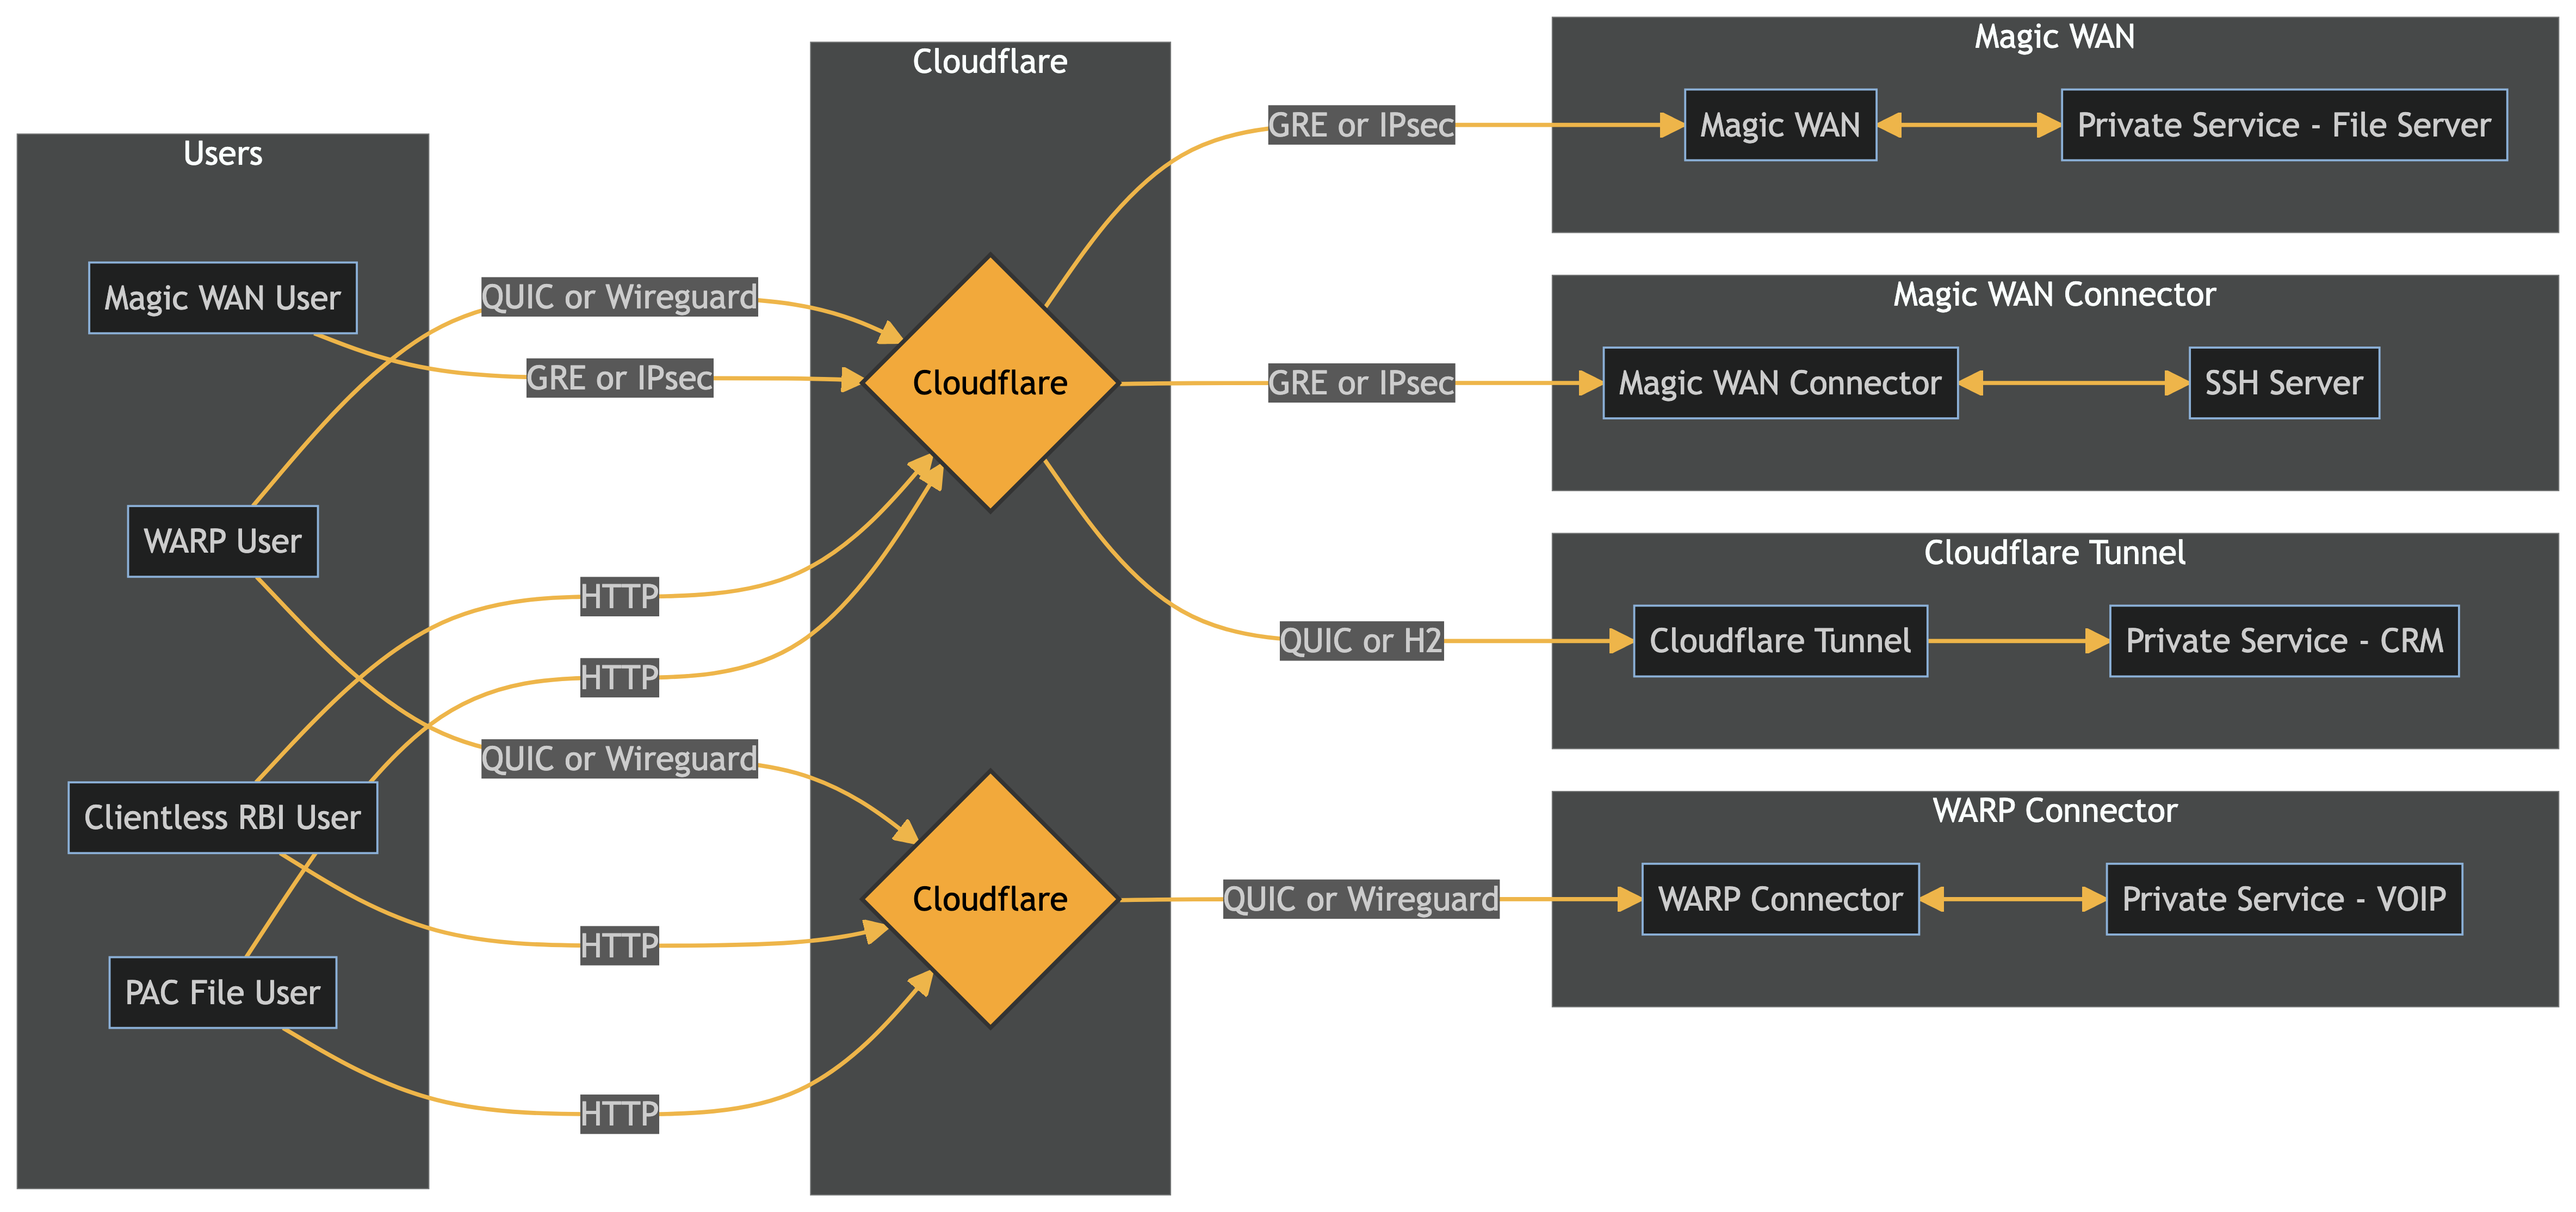
\includegraphics[width=6.5in,height=3.06in]{magic-interop_files/figure-latex/mermaid-figure-1.png}

\footnote{The arrows signify bidirectional connections or unidirectional}

\newpage{}

\paragraph{PAC File (Proxy Endpoints)}\label{pac-file-proxy-endpoints}

There are many ways to deploy the PAC file such as MDMs and using a
remote server, in this case, I'll be using
\href{https://github.com/erfianugrah/worker-proxy-pac}{Workers}. You can
follow the steps
\href{https://developers.cloudflare.com/cloudflare-one/connections/connect-devices/agentless/pac-files/}{here},
when using the code, you can create more cases to match specific files,
in my case it is nl.pac and sg.pac to simulate the two locations, I also
used
\href{https://developers.cloudflare.com/workers/configuration/secrets/}{Workers
Secrets} to store the Proxy Endpoint domains:

\subparagraph{PAC File Worker
Deployment}\label{pac-file-worker-deployment}

Worker entrypoint (index.js)

\begin{Shaded}
\begin{Highlighting}[numbers=left,,]
\ImportTok{import}\NormalTok{ \{ nl\_pac\_file}\OperatorTok{,}\NormalTok{ sg\_pac\_file \} }\ImportTok{from} \StringTok{"./pac\_file.js"}\OperatorTok{;}
 
\ImportTok{export} \ImportTok{default}\NormalTok{ \{}
  \FunctionTok{fetch}\NormalTok{(request}\OperatorTok{,}\NormalTok{ env) \{}
    \KeywordTok{const}\NormalTok{ url }\OperatorTok{=} \KeywordTok{new} \FunctionTok{URL}\NormalTok{(request}\OperatorTok{.}\AttributeTok{url}\NormalTok{)}\OperatorTok{;}
 
    \ControlFlowTok{if}\NormalTok{ (url}\OperatorTok{.}\AttributeTok{pathname} \OperatorTok{===} \StringTok{"/nl.pac"}\NormalTok{) \{}
      \ControlFlowTok{return} \FunctionTok{nl\_pac\_file}\NormalTok{(env)}\OperatorTok{;}
\NormalTok{    \} }\ControlFlowTok{else} \ControlFlowTok{if}\NormalTok{ (url}\OperatorTok{.}\AttributeTok{pathname} \OperatorTok{===} \StringTok{"/sg.pac"}\NormalTok{) \{}
      \ControlFlowTok{return} \FunctionTok{sg\_pac\_file}\NormalTok{(env)}\OperatorTok{;}
\NormalTok{    \} }\ControlFlowTok{else}\NormalTok{ \{}
      \ControlFlowTok{return} \KeywordTok{new} \FunctionTok{Response}\NormalTok{(}\StringTok{"Not Found"}\OperatorTok{,}\NormalTok{ \{ }\DataTypeTok{status}\OperatorTok{:} \DecValTok{404}\NormalTok{ \})}\OperatorTok{;}
\NormalTok{    \}}
\NormalTok{  \}}\OperatorTok{,}
\NormalTok{\}}\OperatorTok{;}
\end{Highlighting}
\end{Shaded}

\newpage{}

PAC File variables (pac\_file.js)

\begin{Shaded}
\begin{Highlighting}[numbers=left,,]
\ImportTok{export} \KeywordTok{function} \FunctionTok{nl\_pac\_file}\NormalTok{(env) \{}
  \KeywordTok{const}\NormalTok{ nl }\OperatorTok{=} \VerbatimStringTok{\textasciigrave{}}
\VerbatimStringTok{function FindProxyForURL(url, host) \{}
\VerbatimStringTok{// No proxy for private (RFC 1918) IP addresses (intranet sites)}
\VerbatimStringTok{  // if (}
\VerbatimStringTok{  //   isInNet(dnsResolve(host), "10.0.0.0", "255.0.0.0") ||}
\VerbatimStringTok{  //   isInNet(dnsResolve(host), "172.16.0.0", "255.240.0.0") ||}
\VerbatimStringTok{  //   isInNet(dnsResolve(host), "192.168.0.0", "255.255.0.0")}
\VerbatimStringTok{  // ) \{}
\VerbatimStringTok{  //   return "DIRECT";}
\VerbatimStringTok{  // \}}
\VerbatimStringTok{ }
\VerbatimStringTok{  // No proxy for localhost}
\VerbatimStringTok{  // if (isInNet(dnsResolve(host), "127.0.0.0", "255.0.0.0")) \{}
\VerbatimStringTok{  //   return "DIRECT";}
\VerbatimStringTok{  // \}}
\VerbatimStringTok{  // Example logic to determine whether to use a proxy}
\VerbatimStringTok{  return "HTTPS }\SpecialCharTok{$\{}\NormalTok{env}\OperatorTok{.}\AttributeTok{NL\_DOMAIN}\SpecialCharTok{\}}\VerbatimStringTok{.proxy.cloudflare{-}gateway.com:443";}
\VerbatimStringTok{\}}
\VerbatimStringTok{\textasciigrave{}}\OperatorTok{;}
  \CommentTok{// Set headers to prevent caching}
  \KeywordTok{const}\NormalTok{ headers }\OperatorTok{=} \KeywordTok{new} \FunctionTok{Headers}\NormalTok{(\{}
    \StringTok{"Content{-}Type"}\OperatorTok{:} \StringTok{"application/x{-}ns{-}proxy{-}auto{-}config"}\OperatorTok{,}
    \StringTok{"Cache{-}Control"}\OperatorTok{:} \StringTok{"no{-}store, max{-}age=0"}\OperatorTok{,}
\NormalTok{  \})}\OperatorTok{;}
 
  \ControlFlowTok{return} \KeywordTok{new} \FunctionTok{Response}\NormalTok{(nl}\OperatorTok{,}\NormalTok{ \{ }\DataTypeTok{headers}\OperatorTok{:}\NormalTok{ headers \})}\OperatorTok{;}
\NormalTok{\}}

\ImportTok{export} \KeywordTok{function} \FunctionTok{sg\_pac\_file}\NormalTok{(env) \{}
  \KeywordTok{const}\NormalTok{ sg }\OperatorTok{=} \VerbatimStringTok{\textasciigrave{}}
\VerbatimStringTok{function FindProxyForURL(url, host) \{}
\VerbatimStringTok{// No proxy for private (RFC 1918) IP addresses (intranet sites)}
\VerbatimStringTok{  // if (}
\VerbatimStringTok{  //   isInNet(dnsResolve(host), "10.0.0.0", "255.0.0.0") ||}
\VerbatimStringTok{  //   isInNet(dnsResolve(host), "172.16.0.0", "255.240.0.0") ||}
\VerbatimStringTok{  //   isInNet(dnsResolve(host), "192.168.0.0", "255.255.0.0")}
\VerbatimStringTok{  // ) \{}
\VerbatimStringTok{  //   return "DIRECT";}
\VerbatimStringTok{  // \}}
\VerbatimStringTok{ }
\VerbatimStringTok{  // No proxy for localhost}
\VerbatimStringTok{  // if (isInNet(dnsResolve(host), "127.0.0.0", "255.0.0.0")) \{}
\VerbatimStringTok{  //   return "DIRECT";}
\VerbatimStringTok{  // \}}
\VerbatimStringTok{  // Example logic to determine whether to use a proxy}
\VerbatimStringTok{  return "HTTPS }\SpecialCharTok{$\{}\NormalTok{env}\OperatorTok{.}\AttributeTok{SG\_DOMAIN}\SpecialCharTok{\}}\VerbatimStringTok{.proxy.cloudflare{-}gateway.com:443";}
\VerbatimStringTok{\}}
\VerbatimStringTok{\textasciigrave{}}\OperatorTok{;}
  \CommentTok{// Set headers to prevent caching}
  \KeywordTok{const}\NormalTok{ headers }\OperatorTok{=} \KeywordTok{new} \FunctionTok{Headers}\NormalTok{(\{}
    \StringTok{"Content{-}Type"}\OperatorTok{:} \StringTok{"application/x{-}ns{-}proxy{-}auto{-}config"}\OperatorTok{,}
    \StringTok{"Cache{-}Control"}\OperatorTok{:} \StringTok{"no{-}store, max{-}age=0"}\OperatorTok{,}
\NormalTok{  \})}\OperatorTok{;}
 
  \ControlFlowTok{return} \KeywordTok{new} \FunctionTok{Response}\NormalTok{(sg}\OperatorTok{,}\NormalTok{ \{ }\DataTypeTok{headers}\OperatorTok{:}\NormalTok{ headers \})}\OperatorTok{;}
\NormalTok{\}}
\end{Highlighting}
\end{Shaded}

\newpage{}

wrangler.toml

\begin{Shaded}
\begin{Highlighting}[numbers=left,,]
\DataTypeTok{name} \OperatorTok{=} \StringTok{"worker{-}proxy{-}pac"}
\DataTypeTok{main} \OperatorTok{=} \StringTok{"src/index.js"}
\DataTypeTok{compatibility\_date} \OperatorTok{=} \StringTok{"2024{-}05{-}12"}
\DataTypeTok{compatibility\_flags} \OperatorTok{=} \OperatorTok{[}\StringTok{"nodejs\_compat"}\OperatorTok{]}
 
\KeywordTok{[dev]}
\DataTypeTok{port} \OperatorTok{=} \DecValTok{9001}
\DataTypeTok{local\_protocol}\OperatorTok{=}\StringTok{"http"}
\DataTypeTok{upstream\_protocol}\OperatorTok{=}\StringTok{"https"}
 
\KeywordTok{[env.staging]}
\DataTypeTok{name} \OperatorTok{=} \StringTok{"staging{-}pac"}
\DataTypeTok{vars} \OperatorTok{=} \OperatorTok{\{ }\DataTypeTok{ENVIRONMENT}\OperatorTok{ =} \StringTok{"staging"}\OperatorTok{ \}}
\DataTypeTok{workers\_dev} \OperatorTok{=} \ConstantTok{true}
 
\KeywordTok{[env.prod]}
\DataTypeTok{name} \OperatorTok{=} \StringTok{"prod{-}pac"}
\DataTypeTok{vars} \OperatorTok{=} \OperatorTok{\{ }\DataTypeTok{ENVIRONMENT}\OperatorTok{ =} \StringTok{"production"}\OperatorTok{ \}}
\DataTypeTok{routes} \OperatorTok{=} \OperatorTok{[}
    \OperatorTok{\{ }\DataTypeTok{pattern}\OperatorTok{ =} \StringTok{"proxy.\{DOMAIN\}.com"}\OperatorTok{, }\DataTypeTok{custom\_domain}\OperatorTok{ =} \ConstantTok{true}\OperatorTok{ \},}
\OperatorTok{]}
\CommentTok{\# Secrets}
\CommentTok{\# NL\_DOMAIN}
\CommentTok{\# SG\_DOMAIN}
\end{Highlighting}
\end{Shaded}

\newpage{}

\subparagraph{Gitops/IaC}\label{gitopsiac}

Proxy Endpoints HCL

\begin{Shaded}
\begin{Highlighting}[numbers=left,,]
\KeywordTok{resource} \StringTok{"cloudflare\_teams\_proxy\_endpoint"} \StringTok{"nl\_proxy\_endpoint"}\NormalTok{ \{}
\NormalTok{  account\_id }\OperatorTok{=} \VariableTok{var}\NormalTok{.cloudflare\_account\_id}
\NormalTok{  name       }\OperatorTok{=} \StringTok{"nl"}
\NormalTok{  ips        }\OperatorTok{=}\NormalTok{ [}\StringTok{"}\SpecialStringTok{$\{}\VariableTok{var.nl\_ip}\SpecialStringTok{\}}\StringTok{/32"}\NormalTok{]}
\NormalTok{\}}
 
\KeywordTok{resource} \StringTok{"cloudflare\_teams\_proxy\_endpoint"} \StringTok{"sg\_proxy\_endpoint"}\NormalTok{ \{}
\NormalTok{  account\_id }\OperatorTok{=} \VariableTok{var}\NormalTok{.cloudflare\_account\_id}
\NormalTok{  name       }\OperatorTok{=} \StringTok{"sg"}
\NormalTok{  ips        }\OperatorTok{=}\NormalTok{ [}\StringTok{"}\SpecialStringTok{$\{}\VariableTok{var.sg\_ip}\SpecialStringTok{\}}\StringTok{/32"}\NormalTok{]}
\NormalTok{\}}
\end{Highlighting}
\end{Shaded}

\paragraph{WARP/Clientless RBI}\label{warpclientless-rbi}

With WARP, the
\href{https://developers.cloudflare.com/cloudflare-one/connections/connect-devices/warp/deployment/mdm-deployment/}{managed}
deployment approach is recommended as you can ensure that not only
you're managing the devices and the policies but also the WARP client
itself. This can also be managed through the use of
\href{https://developers.cloudflare.com/cloudflare-one/connections/connect-devices/warp/configure-warp/device-profiles/}{Device
Profiles}. If the use case is to connect to endpoints behind Cloudflare
Tunnel or Magic WAN, select the \texttt{default}
\href{https://developers.cloudflare.com/cloudflare-one/connections/connect-networks/private-net/cloudflared/tunnel-virtual-networks/}{Virtual
Network} in the client's dropdown menu.

Both WARP (you can also isolate applications) and
\href{https://developers.cloudflare.com/cloudflare-one/policies/browser-isolation/setup/clientless-browser-isolation/\#clientless-web-isolation}{Clientless
RBI} would use the same Access application and policy as shown below,
and both would allow the user to access private IP applications via the
other on-ramps.

\subparagraph{Gitops/Iac}\label{gitopsiac-1}

WARP/RBI Access Policy HCL

\begin{Shaded}
\begin{Highlighting}[numbers=left,,]
\KeywordTok{resource} \StringTok{"cloudflare\_access\_policy"} \StringTok{"warp\_login"}\NormalTok{ \{}
\NormalTok{  account\_id       }\OperatorTok{=} \VariableTok{var}\NormalTok{.cloudflare\_account\_id}
\NormalTok{  name             }\OperatorTok{=} \StringTok{"Allow Erfi"}
\NormalTok{  decision         }\OperatorTok{=} \StringTok{"allow"}
\NormalTok{  session\_duration }\OperatorTok{=} \StringTok{"30m"}
 
\NormalTok{  include \{}
\NormalTok{    group }\OperatorTok{=}\NormalTok{ [cloudflare\_access\_group.erfi\_corp.id]}
\NormalTok{  \}}
\NormalTok{\}}
\end{Highlighting}
\end{Shaded}

\newpage{}

WARP/RBI Access App HCL

\begin{Shaded}
\begin{Highlighting}[numbers=left,,]
\KeywordTok{resource} \StringTok{"cloudflare\_access\_application"} \StringTok{"warp\_login"}\NormalTok{ \{}
\NormalTok{  account\_id }\OperatorTok{=} \VariableTok{var}\NormalTok{.cloudflare\_account\_id}
\NormalTok{  policies }\OperatorTok{=}\NormalTok{ [}
\NormalTok{    cloudflare\_access\_policy.warp\_login.id}
\NormalTok{  ]}
\NormalTok{  allowed\_idps }\OperatorTok{=}\NormalTok{ [}
\NormalTok{    cloudflare\_access\_identity\_provider.entra\_id.id,}
\NormalTok{    cloudflare\_access\_identity\_provider.google\_workspace.id,}
\NormalTok{    cloudflare\_access\_identity\_provider.gmail.id,}
\NormalTok{    cloudflare\_access\_identity\_provider.keycloak\_oidc.id,}
\NormalTok{    cloudflare\_access\_identity\_provider.authentik\_oidc.id,}
\NormalTok{    cloudflare\_access\_identity\_provider.authentik\_saml.id,}
\NormalTok{    cloudflare\_access\_identity\_provider.otp.id}
\NormalTok{  ]}
\NormalTok{  auto\_redirect\_to\_identity }\OperatorTok{=} \VariableTok{false}
\NormalTok{  domain                    }\OperatorTok{=} \StringTok{"erfianugrah.cloudflareaccess.com/warp"}
\NormalTok{  name                      }\OperatorTok{=} \StringTok{"Warp Login App"}
\NormalTok{  session\_duration          }\OperatorTok{=} \StringTok{"24h"}
\NormalTok{  type                      }\OperatorTok{=} \StringTok{"warp"}
\NormalTok{\}}
\end{Highlighting}
\end{Shaded}

Virtual Networks HCL

\begin{Shaded}
\begin{Highlighting}[numbers=left,,]
\KeywordTok{resource} \StringTok{"cloudflare\_tunnel\_virtual\_network"} \StringTok{"vyos\_nl"}\NormalTok{ \{}
\NormalTok{  account\_id }\OperatorTok{=} \VariableTok{var}\NormalTok{.cloudflare\_account\_id}
\NormalTok{  name       }\OperatorTok{=} \StringTok{"vyos\_nl\_vnet"}
\NormalTok{  is\_default\_network }\OperatorTok{=} \VariableTok{true}
\NormalTok{\}}
\end{Highlighting}
\end{Shaded}

\newpage{}

Device Settings Policy HCL

\begin{Shaded}
\begin{Highlighting}[numbers=left,,]
\KeywordTok{resource} \StringTok{"cloudflare\_device\_settings\_policy"} \StringTok{"default"}\NormalTok{ \{}
\NormalTok{  account\_id            }\OperatorTok{=} \VariableTok{var}\NormalTok{.cloudflare\_account\_id}
\NormalTok{  name                  }\OperatorTok{=} \StringTok{"default"}
\NormalTok{  description           }\OperatorTok{=} \StringTok{"default\_policy"}
  \CommentTok{\# precedence            = 100}
  \CommentTok{\# match                 = "any(identity.groups.name[*] in \{\textbackslash{}"Erfi Corp\textbackslash{}"\})"}
\NormalTok{  default               }\OperatorTok{=} \VariableTok{true}
\NormalTok{  enabled               }\OperatorTok{=} \VariableTok{true}
\NormalTok{  allow\_mode\_switch     }\OperatorTok{=} \VariableTok{true}
\NormalTok{  allow\_updates         }\OperatorTok{=} \VariableTok{true}
\NormalTok{  allowed\_to\_leave      }\OperatorTok{=} \VariableTok{true}
\NormalTok{  auto\_connect          }\OperatorTok{=} \DecValTok{0}
\NormalTok{  captive\_portal        }\OperatorTok{=} \DecValTok{180}
\NormalTok{  disable\_auto\_fallback }\OperatorTok{=} \VariableTok{false}
\NormalTok{  switch\_locked         }\OperatorTok{=} \VariableTok{false}
\NormalTok{  service\_mode\_v2\_mode  }\OperatorTok{=} \StringTok{"warp"}
\NormalTok{  service\_mode\_v2\_port  }\OperatorTok{=} \DecValTok{3000}
\NormalTok{  exclude\_office\_ips    }\OperatorTok{=} \VariableTok{true}
\NormalTok{\}}
 
\KeywordTok{resource} \StringTok{"cloudflare\_device\_settings\_policy"} \StringTok{"google"}\NormalTok{ \{}
\NormalTok{  account\_id            }\OperatorTok{=} \VariableTok{var}\NormalTok{.cloudflare\_account\_id}
\NormalTok{  name                  }\OperatorTok{=} \StringTok{"Google Workspace"}
\NormalTok{  description           }\OperatorTok{=} \StringTok{"google\_workspace\_policy"}
\NormalTok{  precedence            }\OperatorTok{=} \DecValTok{200}
\NormalTok{  match                 }\OperatorTok{=} \StringTok{"any(identity.groups.name[*] in \{\textbackslash{}"}\NormalTok{Erfi Corp}\OperatorTok{\textbackslash{}}\StringTok{"\})"}
\NormalTok{  default               }\OperatorTok{=} \VariableTok{false}
\NormalTok{  enabled               }\OperatorTok{=} \VariableTok{true}
\NormalTok{  allow\_mode\_switch     }\OperatorTok{=} \VariableTok{true}
\NormalTok{  allow\_updates         }\OperatorTok{=} \VariableTok{true}
\NormalTok{  allowed\_to\_leave      }\OperatorTok{=} \VariableTok{true}
\NormalTok{  auto\_connect          }\OperatorTok{=} \DecValTok{0}
\NormalTok{  captive\_portal        }\OperatorTok{=} \DecValTok{180}
\NormalTok{  disable\_auto\_fallback }\OperatorTok{=} \VariableTok{false}
\NormalTok{  switch\_locked         }\OperatorTok{=} \VariableTok{false}
\NormalTok{  service\_mode\_v2\_mode  }\OperatorTok{=} \StringTok{"warp"}
\NormalTok{  service\_mode\_v2\_port  }\OperatorTok{=} \DecValTok{3000}
\NormalTok{  exclude\_office\_ips    }\OperatorTok{=} \VariableTok{true}
\NormalTok{\}}
\end{Highlighting}
\end{Shaded}

\newpage{}

\paragraph{Cloudflare Tunnel}\label{cloudflare-tunnel}

Tunnels are used to exposed private applications or for connectivity in
the case of RDP, SSH, VNC and the like, it does not support
bi-directional traffic as mentioned above. By setting up the routes, you
can now reach those same private applications behind Cloudflare Tunnel
be it from a PAC file, clientless RBI, WARP or behind Magic WAN.

\begin{tcolorbox}[enhanced jigsaw, title=\textcolor{quarto-callout-note-color}{\faInfo}\hspace{0.5em}{Note}, rightrule=.15mm, bottomtitle=1mm, opacitybacktitle=0.6, titlerule=0mm, colbacktitle=quarto-callout-note-color!10!white, coltitle=black, opacityback=0, left=2mm, toprule=.15mm, breakable, toptitle=1mm, arc=.35mm, colback=white, bottomrule=.15mm, leftrule=.75mm, colframe=quarto-callout-note-color-frame]

\textbf{Cloudflare Tunnel Deployment}

There are (again) like WARP many ways to deploy, as systemd on a VM or
metal, docker standalone or in compose or a deployment in k8s or docker
swarm.

Be aware of the system requirements:

For most use cases, we recommend the following baseline configuration:

\begin{itemize}
\tightlist
\item
  Run a cloudflared replica on two dedicated host machines per network
  location. Using two hosts enables server-side redundancy and traffic
  balancing.
\item
  Size each host with minimum 4GB of RAM and 4 CPU cores.
\item
  Allocate 50,000 ports to the cloudflared process on each host.
\end{itemize}

This setup is usually sufficient to handle traffic from 8,000 WARP users
(4,000 per host). The actual amount of resources used by cloudflared
will depend on many variables, including the number of requests per
second, bandwidth, network path and hardware. As additional users are
onboarded, or if network traffic increases beyond your existing tunnel
capacity, you can scale your tunnel by adding an additional cloudflared
host in that location.

\end{tcolorbox}

\newpage{}

\subparagraph{Gitops/IaC}\label{gitopsiac-2}

Terraform provider HCL with random provider

\begin{Shaded}
\begin{Highlighting}[numbers=left,,]
\KeywordTok{terraform}\NormalTok{ \{}
  \KeywordTok{required\_providers}\NormalTok{ \{}
\NormalTok{    cloudflare }\OperatorTok{=}\NormalTok{ \{}
      \KeywordTok{source}  \OperatorTok{=} \StringTok{"cloudflare/cloudflare"}
\NormalTok{      version }\OperatorTok{=} \StringTok{"\textasciitilde{}\textgreater{} 4.0"}
\NormalTok{    \}}
\NormalTok{    random }\OperatorTok{=}\NormalTok{ \{}
      \KeywordTok{source}  \OperatorTok{=} \StringTok{"hashicorp/random"}
\NormalTok{      version }\OperatorTok{=} \StringTok{"\textasciitilde{}\textgreater{} 3.0"}
\NormalTok{    \}}
\NormalTok{  \}}
\NormalTok{\}}
\end{Highlighting}
\end{Shaded}

Use the random provider to generate string that will be use to set the
tunnel secret

\begin{Shaded}
\begin{Highlighting}[numbers=left,,]
\CommentTok{\# Generate a random string}
\KeywordTok{resource} \StringTok{"random\_string"} \StringTok{"tunnel\_secret"}\NormalTok{ \{}
  \BuiltInTok{length}  \OperatorTok{=} \DecValTok{32}
\NormalTok{  special }\OperatorTok{=} \VariableTok{false}
\NormalTok{\}}
\end{Highlighting}
\end{Shaded}

Use the random string as the tunnel secret to create the Cloudflare
Tunnel

\begin{Shaded}
\begin{Highlighting}[numbers=left,,]
\KeywordTok{resource} \StringTok{"cloudflare\_tunnel"} \StringTok{"vyos\_nl"}\NormalTok{ \{}
\NormalTok{  account\_id }\OperatorTok{=} \VariableTok{var}\NormalTok{.cloudflare\_account\_id}
\NormalTok{  name       }\OperatorTok{=} \StringTok{"vyos\_nl"}
\NormalTok{  secret     }\OperatorTok{=} \BuiltInTok{base64encode}\NormalTok{(random\_string.tunnel\_secret.result)}
\NormalTok{  config\_src }\OperatorTok{=} \StringTok{"cloudflare"}
\NormalTok{\}}
\end{Highlighting}
\end{Shaded}

\newpage{}

\begin{tcolorbox}[enhanced jigsaw, title=\textcolor{quarto-callout-warning-color}{\faExclamationTriangle}\hspace{0.5em}{Warning}, rightrule=.15mm, bottomtitle=1mm, opacitybacktitle=0.6, titlerule=0mm, colbacktitle=quarto-callout-warning-color!10!white, coltitle=black, opacityback=0, left=2mm, toprule=.15mm, breakable, toptitle=1mm, arc=.35mm, colback=white, bottomrule=.15mm, leftrule=.75mm, colframe=quarto-callout-warning-color-frame]

Again, be aware of conflicting routes between Cloudflare Tunnel and
Magic WAN

\end{tcolorbox}

Tunnel Route HCL

\begin{Shaded}
\begin{Highlighting}[numbers=left,,]
\KeywordTok{resource} \StringTok{"cloudflare\_tunnel\_route"} \StringTok{"vyos\_nl"}\NormalTok{ \{}
\NormalTok{  account\_id         }\OperatorTok{=} \VariableTok{var}\NormalTok{.cloudflare\_account\_id}
\NormalTok{  tunnel\_id          }\OperatorTok{=}\NormalTok{ cloudflare\_tunnel.vyos\_nl.id}
\NormalTok{  network            }\OperatorTok{=} \StringTok{"0.0.0.0/0"}
\NormalTok{  virtual\_network\_id }\OperatorTok{=}\NormalTok{ cloudflare\_tunnel\_virtual\_network.vyos\_nl.id}
\NormalTok{\}}
\end{Highlighting}
\end{Shaded}

Tunnel Config HCL

\begin{Shaded}
\begin{Highlighting}[numbers=left,,]
\KeywordTok{resource} \StringTok{"cloudflare\_tunnel\_config"} \StringTok{"vyos\_nl"}\NormalTok{ \{}
\NormalTok{  account\_id }\OperatorTok{=} \VariableTok{var}\NormalTok{.cloudflare\_account\_id}
\NormalTok{  tunnel\_id  }\OperatorTok{=}\NormalTok{ cloudflare\_tunnel.vyos\_nl.id}
 
\NormalTok{  config \{}
\NormalTok{    warp\_routing \{}
\NormalTok{      enabled }\OperatorTok{=} \VariableTok{true}
\NormalTok{    \}}
\NormalTok{    ingress\_rule \{}
\NormalTok{      hostname }\OperatorTok{=} \StringTok{"prom{-}tunnel{-}nl.}\SpecialStringTok{$\{}\VariableTok{var.domain\_name}\SpecialStringTok{\}}\StringTok{"}
\NormalTok{      service  }\OperatorTok{=} \StringTok{"http://localhost:11000"}
\NormalTok{    \}}
\NormalTok{    ingress\_rule \{}
\NormalTok{      hostname }\OperatorTok{=} \StringTok{"prom{-}caddy{-}nl.}\SpecialStringTok{$\{}\VariableTok{var.domain\_name}\SpecialStringTok{\}}\StringTok{"}
\NormalTok{      service  }\OperatorTok{=} \StringTok{"http://172.18.0.4:2018"}
\NormalTok{    \}}
\NormalTok{    ingress\_rule \{}
\NormalTok{      service }\OperatorTok{=} \StringTok{"http\_status:404"}
\NormalTok{    \}}
\NormalTok{  \}}
\NormalTok{\}}
\end{Highlighting}
\end{Shaded}

\newpage{}

\paragraph{(Beta) WARP Connector}\label{beta-warp-connector}

It shares the same functionality as Cloudflare Tunnel does but with
bidirectional support. This means that only you can expose private
services/applications which require two-way traffic such as
communication services.

As the WARP connector is also essentially a device connected via WARP to
the internet, a remote user with WARP connectivity can also connect to
it directly and not just the services exposed behind it which is what we
call WARP-to-WARP connectivity. Both site-to-site and peer-to-peer use
cases work here, similar to Magic WAN.

\subparagraph{Site-to-site
Connectivity}\label{site-to-site-connectivity}

\begin{enumerate}
\def\labelenumi{\arabic{enumi}.}
\tightlist
\item
  Setup Access policy for WARP enrolment (this would be the same policy
  for WARP authentication), since it's site-to-site, we will have to
  deploy it via \texttt{.xml} with the required parameters.
\end{enumerate}

Refer to
\href{https://developers.cloudflare.com/cloudflare-one/identity/service-tokens/}{service
tokens} and
\href{https://developers.cloudflare.com/cloudflare-one/connections/connect-devices/warp/deployment/device-enrollment/}{device
enrolment} for details.

\begin{enumerate}
\def\labelenumi{\arabic{enumi}.}
\setcounter{enumi}{1}
\tightlist
\item
  Setup the \texttt{split\ tunnel} to either \texttt{include} or
  \texttt{exclude} mode, in this example, I have chosen \texttt{exclude}
  so that I can still SSH into the nodes to showcase the functionality.
\end{enumerate}

Since this portion can be managed by Terraform, this is the example HCL:

\begin{Shaded}
\begin{Highlighting}[numbers=left,,]
\KeywordTok{resource} \StringTok{"cloudflare\_split\_tunnel"} \StringTok{"default\_include"}\NormalTok{ \{}
\NormalTok{  account\_id }\OperatorTok{=} \VariableTok{var}\NormalTok{.cloudflare\_account\_id}
\NormalTok{  policy\_id  }\OperatorTok{=}\NormalTok{ cloudflare\_device\_settings\_policy.default.id}
\NormalTok{  mode       }\OperatorTok{=} \StringTok{"exclude"}
\NormalTok{  tunnels \{}
\NormalTok{    address     }\OperatorTok{=} \StringTok{"10.68.69.3"}
\NormalTok{    description }\OperatorTok{=} \StringTok{"ERFI1"}
\NormalTok{  \}}
\NormalTok{  tunnels \{}
\NormalTok{    address     }\OperatorTok{=} \StringTok{"10.68.73.3"}
\NormalTok{    description }\OperatorTok{=} \StringTok{"arch{-}0"}
\NormalTok{  \}}
\NormalTok{  tunnels \{}
\NormalTok{    address     }\OperatorTok{=} \StringTok{"10.68.73.2"}
\NormalTok{    description }\OperatorTok{=} \StringTok{"pve"}
\NormalTok{  \}}
\NormalTok{\}}
\end{Highlighting}
\end{Shaded}

\newpage{}

\begin{enumerate}
\def\labelenumi{\arabic{enumi}.}
\setcounter{enumi}{2}
\tightlist
\item
  Ensure these settings are enabled:
\end{enumerate}

\begin{itemize}
\tightlist
\item
  Enable CGNAT routing (Settings -\textgreater{} Network)

  \begin{itemize}
  \tightlist
  \item
    Enable Proxy (UDP, TCP, ICMP)
  \item
    Enable WARP to WARP
  \item
    Override local interface IP (Settings -\textgreater{} WARP Client)

    \begin{itemize}
    \tightlist
    \item
      If in \texttt{include} mode, ensure \texttt{100.96.0.0/12} is
      included
    \end{itemize}
  \end{itemize}
\end{itemize}

Some of these settings are available as a Terraform resource (as shown
below), since it would be a mix a of API/UI and Terraform, Terraform
would not know the state, so just keep to API/UI for all settings.

\begin{Shaded}
\begin{Highlighting}[numbers=left,,]
\KeywordTok{resource} \StringTok{"cloudflare\_teams\_account"} \StringTok{"miau3"}\NormalTok{ \{}
\NormalTok{  account\_id                             }\OperatorTok{=} \VariableTok{var}\NormalTok{.cloudflare\_account\_id}
\NormalTok{  tls\_decrypt\_enabled                    }\OperatorTok{=} \VariableTok{false}
\NormalTok{  protocol\_detection\_enabled             }\OperatorTok{=} \VariableTok{false}
\NormalTok{  activity\_log\_enabled                   }\OperatorTok{=} \VariableTok{true}
\NormalTok{  non\_identity\_browser\_isolation\_enabled }\OperatorTok{=} \VariableTok{true}

\NormalTok{  body\_scanning \{}
\NormalTok{    inspection\_mode }\OperatorTok{=} \StringTok{"deep"}
\NormalTok{  \}}

\NormalTok{  antivirus \{}
\NormalTok{    enabled\_download\_phase }\OperatorTok{=} \VariableTok{false}
\NormalTok{    enabled\_upload\_phase   }\OperatorTok{=} \VariableTok{false}
\NormalTok{    fail\_closed            }\OperatorTok{=} \VariableTok{false}
\NormalTok{  \}}

\NormalTok{  fips \{}
\NormalTok{    tls }\OperatorTok{=} \VariableTok{false}
\NormalTok{  \}}

\NormalTok{  proxy \{}
\NormalTok{    tcp     }\OperatorTok{=} \VariableTok{true}
\NormalTok{    udp     }\OperatorTok{=} \VariableTok{true}
\NormalTok{    root\_ca }\OperatorTok{=} \VariableTok{true}
\NormalTok{  \}}

\NormalTok{  url\_browser\_isolation\_enabled }\OperatorTok{=} \VariableTok{true}

\NormalTok{  logging \{}
\NormalTok{    redact\_pii }\OperatorTok{=} \VariableTok{false}
\NormalTok{    settings\_by\_rule\_type \{}
\NormalTok{      dns \{}
\NormalTok{        log\_all    }\OperatorTok{=} \VariableTok{true}
\NormalTok{        log\_blocks }\OperatorTok{=} \VariableTok{false}
\NormalTok{      \}}
\NormalTok{      http \{}
\NormalTok{        log\_all    }\OperatorTok{=} \VariableTok{true}
\NormalTok{        log\_blocks }\OperatorTok{=} \VariableTok{false}
\NormalTok{      \}}
\NormalTok{      l4 \{}
\NormalTok{        log\_all    }\OperatorTok{=} \VariableTok{true}
\NormalTok{        log\_blocks }\OperatorTok{=} \VariableTok{false}
\NormalTok{      \}}
\NormalTok{    \}}
\NormalTok{  \}}

\NormalTok{  extended\_email\_matching \{}
\NormalTok{    enabled }\OperatorTok{=} \VariableTok{true}
\NormalTok{  \}}
\NormalTok{\}}
\end{Highlighting}
\end{Shaded}

\begin{enumerate}
\def\labelenumi{\arabic{enumi}.}
\setcounter{enumi}{3}
\tightlist
\item
  Set up the WARP Connector
\end{enumerate}

\begin{itemize}
\tightlist
\item
  Either via API or the UI, create the WARP connector (currently not
  available as a Terraform resource):
\end{itemize}

\begin{Shaded}
\begin{Highlighting}[numbers=left,,]
\NormalTok{curl {-}{-}request POST \textbackslash{}}
\NormalTok{  {-}{-}url https://api.cloudflare.com/client/v4/accounts/account\_id/warp\_connector \textbackslash{}}
\NormalTok{  {-}{-}header \textquotesingle{}Content{-}Type: application/json\textquotesingle{} \textbackslash{}}
\NormalTok{  {-}{-}header \textquotesingle{}X{-}Auth{-}Email: \textquotesingle{} \textbackslash{}}
\NormalTok{  {-}{-}data \textquotesingle{}\{}
\NormalTok{  "name": "arch{-}0"}
\NormalTok{\}\textquotesingle{}}
\end{Highlighting}
\end{Shaded}

Upon creation, you will get the example \texttt{.xml} e.g.~which will
look like this:

\begin{Shaded}
\begin{Highlighting}[numbers=left,,]
\NormalTok{\textless{}}\KeywordTok{dict}\NormalTok{\textgreater{}}
\NormalTok{ \textless{}}\KeywordTok{key}\NormalTok{\textgreater{}organization\textless{}/}\KeywordTok{key}\NormalTok{\textgreater{}}
\NormalTok{ \textless{}}\KeywordTok{string}\NormalTok{\textgreater{}org\_name\textless{}/}\KeywordTok{string}\NormalTok{\textgreater{}}
\NormalTok{ \textless{}}\KeywordTok{key}\NormalTok{\textgreater{}auth\_client\_id\textless{}/}\KeywordTok{key}\NormalTok{\textgreater{}}
\NormalTok{ \textless{}}\KeywordTok{string}\NormalTok{\textgreater{}client\_access\_id\_string\textless{}/}\KeywordTok{string}\NormalTok{\textgreater{}}
\NormalTok{ \textless{}}\KeywordTok{key}\NormalTok{\textgreater{}auth\_client\_secret\textless{}/}\KeywordTok{key}\NormalTok{\textgreater{}}
\NormalTok{ \textless{}}\KeywordTok{string}\NormalTok{\textgreater{}client\_access\_secret\_string\textless{}/}\KeywordTok{string}\NormalTok{\textgreater{}}
\NormalTok{ \textless{}}\KeywordTok{key}\NormalTok{\textgreater{}warp\_connector\_token\textless{}/}\KeywordTok{key}\NormalTok{\textgreater{}}
\NormalTok{ \textless{}}\KeywordTok{string}\NormalTok{\textgreater{}connector\_token\_string\textless{}/}\KeywordTok{string}\NormalTok{\textgreater{}}
\NormalTok{\textless{}/}\KeywordTok{dict}\NormalTok{\textgreater{}}
\end{Highlighting}
\end{Shaded}

This is what you will place in the \texttt{/var/lib/cloudflare-warp}
directory after the WARP client install. Refer to the relevant
\href{https://pkg.cloudflareclient.com/}{repositories} that matches your
Linux distribution, for Arch, you would have to install via
\href{https://aur.archlinux.org/packages/cloudflare-warp-bin}{AUR}.

Once done, if not yet enabled, run
\texttt{sudo\ systemctl\ enable\ warp-svc} then
\texttt{sudo\ systemctl\ start\ warp-svc}, if already running as a
service, run \texttt{sudo\ systemctl\ restart\ warp-svc} so that it will
use the new configuration to connect to Cloudflare.

\newpage{}

\begin{enumerate}
\def\labelenumi{\arabic{enumi}.}
\setcounter{enumi}{4}
\tightlist
\item
  Set up Linux networking
\end{enumerate}

We need to enable IP forwarding and MSS clamping (WARP's MTU is 1280
bytes).

Create a \texttt{.conf} file in the \texttt{etc/sysctl.d/} directory
with value of \texttt{net.ipv4.ip\_forward\ =\ 1} so that this persists
upon reboot.

To check what IPtables rules are existing, we can run
\texttt{sudo\ iptables-save\ \textgreater{}\ test.conf} to just see
what's currently being use, if all's well. We can add the following to
the existing \texttt{/etc/iptables/iptables.rules} file, such that it
would look something like this:

\begin{Shaded}
\begin{Highlighting}[numbers=left,,]
\ExtensionTok{*filter}
\ExtensionTok{:INPUT}\NormalTok{ ACCEPT }\PreprocessorTok{[}\SpecialStringTok{0:0}\PreprocessorTok{]}
\ExtensionTok{:FORWARD}\NormalTok{ ACCEPT }\PreprocessorTok{[}\SpecialStringTok{0:0}\PreprocessorTok{]}
\ExtensionTok{:OUTPUT}\NormalTok{ ACCEPT }\PreprocessorTok{[}\SpecialStringTok{0:0}\PreprocessorTok{]}
\ExtensionTok{{-}A}\NormalTok{ FORWARD }\AttributeTok{{-}i}\NormalTok{ CloudflareWARP }\AttributeTok{{-}p}\NormalTok{ tcp }\AttributeTok{{-}m}\NormalTok{ tcp }\AttributeTok{{-}{-}tcp{-}flags}\NormalTok{ SYN,RST SYN }\AttributeTok{{-}j}\NormalTok{ TCPMSS }\AttributeTok{{-}{-}clamp{-}mss{-}to{-}pmtu}
\ExtensionTok{{-}A}\NormalTok{ FORWARD }\AttributeTok{{-}o}\NormalTok{ CloudflareWARP }\AttributeTok{{-}p}\NormalTok{ tcp }\AttributeTok{{-}m}\NormalTok{ tcp }\AttributeTok{{-}{-}tcp{-}flags}\NormalTok{ SYN,RST SYN }\AttributeTok{{-}j}\NormalTok{ TCPMSS }\AttributeTok{{-}{-}clamp{-}mss{-}to{-}pmtu}
\ExtensionTok{COMMIT}
\end{Highlighting}
\end{Shaded}

This would make sure the MSS clamping rules will also persist on reboot.

\newpage{}

\begin{enumerate}
\def\labelenumi{\arabic{enumi}.}
\setcounter{enumi}{5}
\tightlist
\item
  Route nodes/VMs/containers to the WARP connector
\end{enumerate}

The most common use case here would either be an alternate gateway to
the main router or an intermediate gateway. In this example, I will be
using it as an intermediate gateway.

Set up the \texttt{static\ routes} for each WARP connector, the
configuration will be similar to the \texttt{Cloudflare\ Tunnel} routes.
In our case, on the WARP connector called \texttt{arch-1}, we will
exposing \texttt{10.68.73.102/32} for the \texttt{arch-2} machine, and
\texttt{arch-3} will be exposing \texttt{10.68.73.104/32} for
\texttt{arch-4} machine.

Let's use \texttt{arch-2} as an example as the same steps will be
replicated on the other node.

Run:

\begin{Shaded}
\begin{Highlighting}[numbers=left,,]
\ExtensionTok{ip}\NormalTok{ route}
\end{Highlighting}
\end{Shaded}

and you should be able to see default routes, for instance:

\begin{Shaded}
\begin{Highlighting}[numbers=left,,]
\ExtensionTok{default}\NormalTok{ via 10.68.73.1 dev ens18 proto dhcp src 10.68.73.102 metric 100}
\end{Highlighting}
\end{Shaded}

we want to create another route that has higher precedence than this
(lower number).

Run:

\begin{Shaded}
\begin{Highlighting}[numbers=left,,]
\FunctionTok{sudo}\NormalTok{ ip route add default via 10.68.73.101 dev ens18 metric 99}
\end{Highlighting}
\end{Shaded}

What this means is that, traffic from \texttt{arch-2} will go via the
\texttt{ens18} interface to \texttt{10.68.73.101} which is the WARP
connector \texttt{arch-1} and using it as a gateway, now this node is
connected to Cloudflare.

Do the same for the other node, and change the IP.

Run:

\begin{Shaded}
\begin{Highlighting}[numbers=left,,]
\ExtensionTok{curl}\NormalTok{ https://icanhazip.com}
\end{Highlighting}
\end{Shaded}

on either machine, and you should be able to see a Cloudflare IP, just
be aware since all traffic is sent to the WARP connector, that the DNS
server used by the machines routed to WARP connector can be accessed
while on the network, either by another route or a public DNS server.

\begin{Shaded}
\begin{Highlighting}[numbers=left,,]
\ExtensionTok{curl}\NormalTok{ icanhazip.com                                                              }
\ExtensionTok{104.28.218.39}
\end{Highlighting}
\end{Shaded}

\begin{enumerate}
\def\labelenumi{\arabic{enumi}.}
\setcounter{enumi}{6}
\tightlist
\item
  Route the machines to each other
\end{enumerate}

We can either router the entire prefix to the WARP connector or specific
IPs, in my case, I will be using just one IP:

\begin{Shaded}
\begin{Highlighting}[numbers=left,,]
\FunctionTok{sudo}\NormalTok{ ip route add 10.68.73.104 via 10.68.73.101 dev ens18 metric 98}
\end{Highlighting}
\end{Shaded}

This will allow \texttt{10.68.73.102} to reach \texttt{10.68.73.104}, do
the same on \texttt{arch-4}, just by swapping the IPs, from
\texttt{.104} to \texttt{.102}

Run:

\begin{Shaded}
\begin{Highlighting}[numbers=left,,]
\FunctionTok{ping}\NormalTok{ 10.68.73.102}
\end{Highlighting}
\end{Shaded}

or

\begin{Shaded}
\begin{Highlighting}[numbers=left,,]
\ExtensionTok{mtr}\NormalTok{ 10.68.73.102}
\end{Highlighting}
\end{Shaded}

and vice versa to see the traffic reach the WARP connector CGNAT IP
before reaching the other machine.




\end{document}
